\documentclass[11pt]{IEEEtran}


% Symbol and math packages
\usepackage{gensymb}
\usepackage{amssymb}
\usepackage{amsmath}

% Algorithm packages
\usepackage{algorithm}
\usepackage{algorithmicx}
\usepackage[noend]{algpseudocode}

% Figure, graphics and float packages
\usepackage{cite}
\usepackage{graphicx}
\usepackage{float}
\usepackage{stfloats}

% Paper format packages
\usepackage{multicol}
\usepackage[margin=.9in]{geometry}
\usepackage[font=scriptsize,labelfont=bf]{caption}

\usepackage{setspace}
\usepackage{enumitem}

\setlength{\parskip}{0pt}
\setlist{topsep=11pt, leftmargin=*}

% Set the line spacing
\onehalfspacing

\begin{document}

% Rename algorithmic pre/post condition labels
\renewcommand{\algorithmicrequire}{\textbf{Input:}}
\renewcommand{\algorithmicensure}{\textbf{Output:}}


% Turn off two column for the title and abstract
\twocolumn[ \begin{@twocolumnfalse}
		
% Title
\title{Spiral Packing}
\author{Adrian Cortez \\
	Rochester Institute of Technology \\
	\small \texttt{arc6210@rit.edu}}
\date{May 2015}
\maketitle
	
% Abstract	
\begin{abstract}
Cameron Browne and Paul van Wamelen present a simple iterative method for creating artistic, space-filling designs based on spiral packings, utilizing circle approximations to significantly simplify the spiral packing problem.\cite{Browne2006834} In this paper we implement the algorithm described by Browne and van Wamelen, discuss the underlying geometry in detail and provide a number of color examples generated by the algorithm. The resulting images are evaluated based on how well they are packed and on aspects of their overall design. We show that the algorithm provides a good approximation and generates designs that are both space-filling and visually pleasing.
\break \break
\end{abstract}

\end{@twocolumnfalse}]


% Introduction
\section{Introduction}
\label{introduction}
Spiral packing is the process of filling a given area, or shape boundary, with connected sets of spirals. The sets are generated by successively branching child spirals from parent spirals, constrained to fit nearby neighbors in their environment. This process continues until the area is filled to some desired level of coverage. The ultimate goal is to generate designs that are artistic and space-filling. Examples of generated images using the spiral packing algorithm are shown in Figure~\ref{fig:example}.

\begin{figure}[h]
\centering 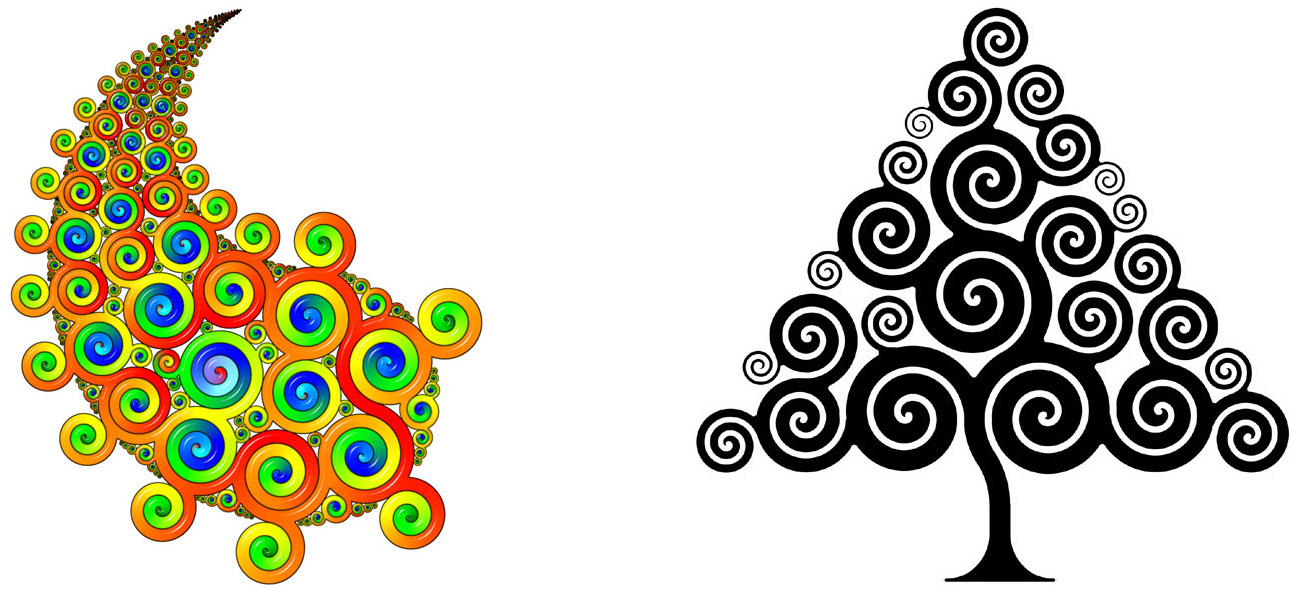
\includegraphics[width=0.9\linewidth]{spiral-packing-example}
\caption{Examples of spiral packing. \cite{Browne2006834}}
\label{fig:example}
\end{figure}

\subsection{Archimedes' Spiral}	
The general polar equation for the Archimedean spiral is 
\begin{equation} 
\label{eq:1} 
	r(\theta) = a\theta^\frac{1}{n} 
\end{equation}

The implemented algorithm utilizes the special case of the Archimedean spiral ($n=1$), known as Archimedes' spiral (Figure~\ref{fig:spiral}, left), described by the equation $ r = a\theta $. This special case was chosen by the authors because of its aesthetic and well-behaved mathematical qualities.\cite{Browne2006834}
	
\begin{figure}[h]
\centering
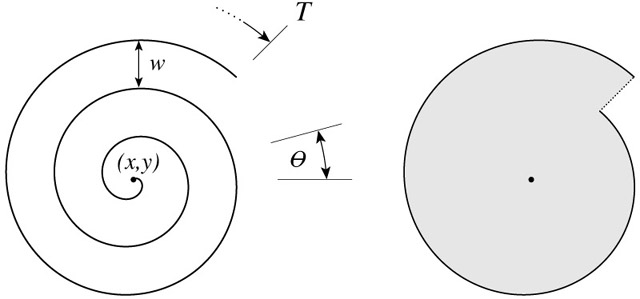
\includegraphics[width=0.9\linewidth]{spiral-packing-fig-02}
\caption{Archimedes's spiral and its footprint. \cite{Browne2006834}}
\label{fig:spiral}
\end{figure}

\begin{figure*}[b!]
\centering
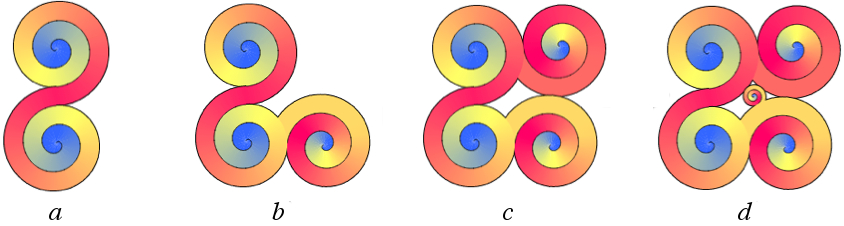
\includegraphics[width=0.75\textwidth]{spiral-branching}
\caption{A simple example of the packing process. The process starts with a pair of seed spirals. Child spirals are then successively branched from the parent spirals, fitting to any potentially intersecting neighbors.}
\label{fig:branch}
\end{figure*}

The Archimedes' spiral can be described in cartesian coordinates by the set of parameters $(x,y,w,\theta,T,\omega)$, giving the parametric equations:
\begin{equation} 
\label{eq:2} 
	x_{s}(t) = x + wt cos(\theta + 2\pi\omega t)
\end{equation}
\begin{equation}
\label{eq:3} 
	y_{s}(t) = y + wt sin(\theta + 2\pi\omega t) 
\end{equation}
for $0 \leq t \leq T$, where $(x,y)$ is the spiral's center, $w$ is the width of one rotation, $\theta$ is the starting angle or phase, $T$ is the number of rotations or total sweep of the spiral, and $\omega$ is the orientation of the spiral ($\omega = -1$ for clockwise and $\omega = 1$ for counterclockwise).

The area enclosed by the outer 360\degree\ sweep of a spiral is described as its footprint (Figure~\ref{fig:spiral}, right). The equation for finding the area bounded by a curve in polar coordinates is 
\begin{equation} \label{eq:4}
	A_{s} = \frac{1}{2} \int_{a}^{b} r(\theta)^2 d\theta
\end{equation}
By using the polar form of the spiral (equation \ref{eq:1}) with $ n = 1 $ and $w = {2 \pi a}$  we can calculate the area of the footprint, and therefore the area of the spiral, as
\begin{equation} 
\label{eq:5} 
\begin{split}
	A_{s} &= \frac{1}{2} \int_{2 \pi (T-1)}^{2 \pi T} (a\theta)^2 d\theta \\
		 &= \frac{4 \pi^3 a^2}{3} (T^3 - (T-1)^3) \\
		 &= \frac{\pi w^2}{3} (T^3 - (T-1)^3) 
\end{split} 
\end{equation}
Notice that the bounds of the integral span from from $ T-1 $ to $ T $, corresponding to the outer turn of the spiral. This is necessary to avoid counting some regions of the spiral area multiple times.

\subsection{Spiral Packing}
\label{spiralpacking}
The goal is to pack a given area with connected sets of Archimedes' spirals. The packing process begins with one or more pairs of seed spirals from which child spirals are successively branched. The seed spirals are generated as a pair of opposed matching spirals, $S_{1}$ and $S_{2}$. The seed spirals have identical $ w, T, \omega $, opposed $\theta$ and are oriented with tangential endpoints such that $ x_{s_{1}}(T) = x_{s_{2}}(T-1) $, 
$ y_{s_{1}}(T) = y_{s_{2}}(T-1)$, 
$ x_{s_{1}}(T-1) = x_{s_{2}}(T)$, and 
$ y_{s_{1}}(T-1) = y_{s_{2}}(T) $. 
This relationship is shown in Figure~\ref{fig:branch}a. This process continues by branching child spirals from parent spirals until the target area is packed to some desired density. 

The term \textit{connected spiral set} is used to describe the collection of spirals that ultimately branch from a single seed pair. This means that there will be as many spiral sets as there are seed pairs. The defining property of connected spiral sets is that every interior point within the set is connected to every other. When generating connected spiral sets, the following constraints must not be violated:
\begin{enumerate}
	\item A child must have only one parent, though parents may have multiple children,
	
	\item A child must not have a greater width $w$ than its parent,
  	
	\item Each child must meet its parent tangentially,
  	
	\item Each child must be rotated such that its terminal point lies on the line drawn between its center and its parent's center, and
  	
	\item Spirals may touch neighboring spirals tangentially but may not intersect them.
\end{enumerate}

Figure~\ref{fig:branch} demonstrates a simple example of the packing process. The process starts with a seed pair (Fig.~\ref{fig:branch}a) from which a single child spiral branches (Fig.~\ref{fig:branch}b). Then an additional child spiral is branched, touching one neighboring spiral tangentially (Fig.~\ref{fig:branch}c). A final child spiral is then placed, its width constrained (lessened) so that it touches the two neighboring spirals without intersecting them (Fig.~\ref{fig:branch}d).

\begin{figure*}[t]
\centering 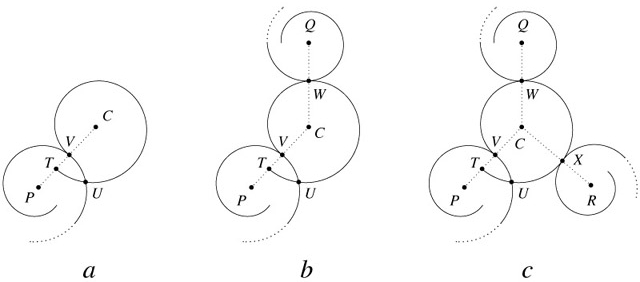
\includegraphics[width=0.75\textwidth]{spiral-packing-fig-01}
\caption{The three geometric cases when branching: (a) simple branching, (b) fitting a child spiral to one neighboring spiral, and (c) fitting a child spiral to two neighboring spirals. \cite{Browne2006834}}
\label{fig:geo}
\end{figure*}

The underlying geometry that captures these constraints can be described in three general cases, as shown in Figure~\ref{fig:geo}. 

\begin{enumerate}
	\item \textit{Case I}: The most simple branching case. A child spiral $S$, branching from an existing parent spiral $S_{1}$, is placed in such a way that it does not intersect any neighboring spirals (Fig~\ref{fig:geo}a). This is handled simply by drawing $S$ at the specified location. 
	
	\item \textit{Case II}: A child spiral $S$, branching from an existing parent spiral $S_{1}$, is placed so that it intersects one neighboring spiral, $S_{2}$ (Fig~\ref{fig:geo}b). $S$ must be repositioned, resized, or both so that it lies tangent to $S_{2}$.
	
	\item \textit{Case III}: A child spiral $S$, branching from an existing parent spiral $S_{1}$, is placed so that it intersects two neighboring spirals, $S_{2}$ and  $S_{3}$ (Fig~\ref{fig:geo}c). $S$ must be repositioned, resized, or both so that it lies tangent to both $S_{2}$ and  $S_{3}$. 
\end{enumerate}

In the case where two neighboring spirals are intersected, there is a possibility that the algorithm may not converge in a way to allow the child spiral to lie tangent to both neighbors. In this case, the maximally intersected neighbor is chosen as the spiral to position the child spiral tangent to.

In all cases, the child spiral $S$ is rotated to lie tangent to the parent spiral $S_{1}$ such that its end point $T$ lies on the line between the spiral centers. $S$ is clipped at the intersection point $U$ and $S_{1}$ is clipped along the interval between the tangent point $V$ and intersection point $U$. The parent spiral is considered a complete spiral even though intervals along its sweep may be clipped by children.

\subsection{Numerical Solution and Circle Approximations}	
The problem of packing spirals is a difficult problem to solve numerically. Consider the solution of case III, which is the most difficult of the three geometric cases. There are a total of ten variables in cartesian coordinates that need to be solved for:
\begin{enumerate}
\item $x$, $y$, $w$ and $\theta$ of the child spiral we are trying to place,
\item $t_{i}$ and $t^{\prime}_{i}$ are the real numbers where the child  spiral $S$ at $t_{i}$ touches a neighboring spiral $S_{i}$ at $t^{\prime}_{i}$ for $i = 1,2,3$.
\end{enumerate}

Solving for these ten variables simultaneously requires a system of ten equations that describe the relevant intersections and tangential points. A system this complex has to be solved numerically and one of the simplest methods to do so is the Newton's Method for Systems. Defining the ten variables as a vector $\textit{\textbf{v}} = (x, y, w, \theta, t_{1}, t_{2}, t_{3}, t^{\prime}_{1}, t^{\prime}_{2}, t^{\prime}_{3})$ and the ten equations as a column vector $\textit{F}(\textbf{v}) = (\textit{f}_{1}(\textbf{v}), \textit{f}_{2}(\textbf{v}),...,\textit{f}_{10}(\textbf{v}))$ leads to the system 
\begin{equation} 
	\label{eq:6}
	\boldsymbol{v}_{i+1} = \boldsymbol{v}_{i} - J(\boldsymbol{v}_{i})^{-1}F(\boldsymbol{v}_{i})
\end{equation}
Where $\textit{J}(\textbf{v})$ is the $10\times10$ Jacobian matrix. The solutions for cases I and II require similar, but simplified, systems of equations to be solved. Browne and van Wamelen explain the process of solving these systems of equations in more detail\cite{Browne2006834}. 

Though the process of solving these systems of equations is relatively straightforward, it is difficult and rather tedious. This created the motivation for a simpler method of achieving spiral packings. By exploring the related study of circle packing, Browne and van Wamelen devised an iterative method for packing spirals using circles to approximate the spirals. At each iteration the solution is refined by making better circle approximations.\cite{Browne2006834}

Circle packing, also known as Apollonian packing, is the class of problems of drawing a circle tangent to three other objects where each of these objects could be either a point, line or circle. It was first described by the Greek mathematician Apollonius of Perga in the 3rd century BC. There are a total of ten different cases to the circle packing problem.\cite{Bourke2006} For the purposes of simplifying the spiral packing process, we are interested only in the solution to the last of the ten cases; the problem of fitting a circle tangent to three other circles, known as Apollonius' Tenth problem (Figure~\ref{fig:circle}). In particular, we are interested in the solution that yields the minimum radius.\cite{Browne2006834} By approximating the spirals as circles the spiral packing problem is reduced to the circle packing problem of interest. This significantly simplifies the process of fitting a child spiral to neighboring spirals.

\begin{figure}[h!]
\centering 
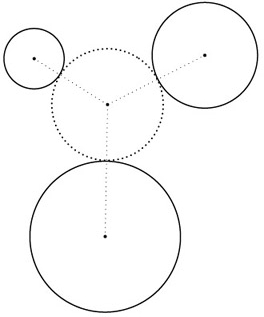
\includegraphics[width=0.5\linewidth]{spiral-circles}
\caption{Apollonian packing for the case of one circle fitting tangent to three other circles.\cite{Browne2006834}}
\label{fig:circle}
\end{figure}

There are obvious similarities between the packing of circles and the packing of spirals. However, there are differences that make spiral packing a more difficult problem to solve. With that said, the solution to the circle packing problem provides a good framework on which to build a robust approximate solution to achieve the spiral packing that is desired.\cite{Browne2006834}.


% Implementation
\section{Implementation}
\label{implementation}
To begin generating connected spiral sets, the implemented program starts with one or more pairs of seed spirals from which the child spirals can branch. During the branching process, the user provides a the number of turns, orientation, preferred location for the child spiral to place. The algorithm takes the these parameters, in conjunction with the constraints listed above and the state of the packed area, to attempt to place the child spiral. The goal is to place the child spiral as close to the user's preferred location as possible without violating the constraints. In addition, the algorithm must be robust enough to handle ambiguous child placements by the user.

In order to place a child spiral we must first be able to solve geometric cases I, II, and III of the fitting problem described in Section~\ref{introduction}. This is an iterative process that approximates the input spirals as circles and solves the appropriate circle packing problem. The fitting algorithm for all three cases is as follows:
\begin{enumerate}
	\item Approximate the spirals as circles,
	\item Solve the appropriate circle fitting problem, and
	\item Use the solution to make better approximations to the spirals.
\end{enumerate}
Pseudocode for this procedure is shown in Algorithm~\ref{alg:fitting} in Appendix A. 
	
The general fitting algorithm attempts to find a child spiral $S$ branching from a parent spiral $S_{1}$ as close to the preferred location specified by the user while being fitted to any potentially intersecting spirals, $S_{2}$ and $S_{3}$. Therefore the algorithm requires a parent spiral $S_{1}$ and a child spiral $S_{0}$ with a specified number of turns $T$, orientation $\omega$, and a preferred location $(x, y)$ as input. Pseudocode for the general algorithm is given in Algorithm~\ref{alg:branch} in Appendix A, however, it is simply stated as follows:
\begin{enumerate}
	\item If $S_{0}$ does not intersect other spirals let $S = S_{0}$.
	\item If $S_{0}$ intersects two or more spirals, then try to fit S to the closest two without being too far from $S_{0}$.
	\item If Step 2. fails or there is only one intersecting spiral, then try to fit a spiral with the same width as $S_{0}$ to the spiral with the greatest intersection with $S_{0}$. If the resulting spiral is close enough to $(x, y)$ then use it.
	\item If all else fails fit the biggest spiral in the direction of $S_{0}$ to the parent.
\end{enumerate}

The algorithms described were implemented using JavaScript, HTML and SVG and was design to be able to run in the browser. The program has two basic operations: placing a seed spiral and branching a child spiral from a parent spiral.

The user interactively specifies the preferred location of each seed pair or child using the mouse. The program adds the correctly fitted result if possible. The degrees of freedom for the spirals (width, number of turns, orientation and so on) are specified globally and can be edited by the user. Any placed spiral may be deleted.

The program also allows the user to specify the color for each spiral. A user may choose up to six colors. If multiple colors are given, then the colors are blended into a gradient that is applied along the spiral's path. 

Since the aesthetic value of the color is evaluated by the program, the user is given multiple options for generating harmonious color schemes. The simplest option provided is to use one of the three color sets that make up the color wheel. These are the \textit{primary}, \textit{secondary}, and \textit{tertiary} colors. For more complex color schemes, the user can specify a basis color and have a color combination generated for them. The program can generate color combinations using the following techniques\cite{quiller2002}: 
\begin{itemize}
	\item \textit{Complementary} - Colors that are opposite each other on the color wheel. Generates a two-color scheme.
	\item \textit{Split-complementary} - A variation of the complementary color scheme. In addition to the base color, it uses the two colors adjacent to its complement. Generates a three-color scheme.
	\item \textit{Analogous} - Colors that are next to each other on the color wheel. Generates a three-color scheme.
	\item \textit{Triadic} - Colors that are evenly spaced around the color wheel. Generates a three-color scheme.
	\item \textit{Tetradic} - Uses four colors arranged into two complementary pairs. Generates a four-color scheme.
	\item \textit{Monochromatic} - Colors that are fairly similar to each other derived from a single hue. Generates a five-color scheme.
\end{itemize}

Boundary shapes were implemented in the program as sets of small, closely spaced spirals laid along the boundary path. Boundary spirals have very small widths and a large number of turns to give them reasonably constant exterior curvature and make them circle-like in nature. This conveniently allowed the algorithm to also handle fitting to the boundary shapes. The spirals that make up the boundary shapes are excluded from the final output.

% Results
\section{Results}
The following images were generated using the implemented program. Larger versions are shown in Appendix B. 

\begin{figure}[h]
\centering 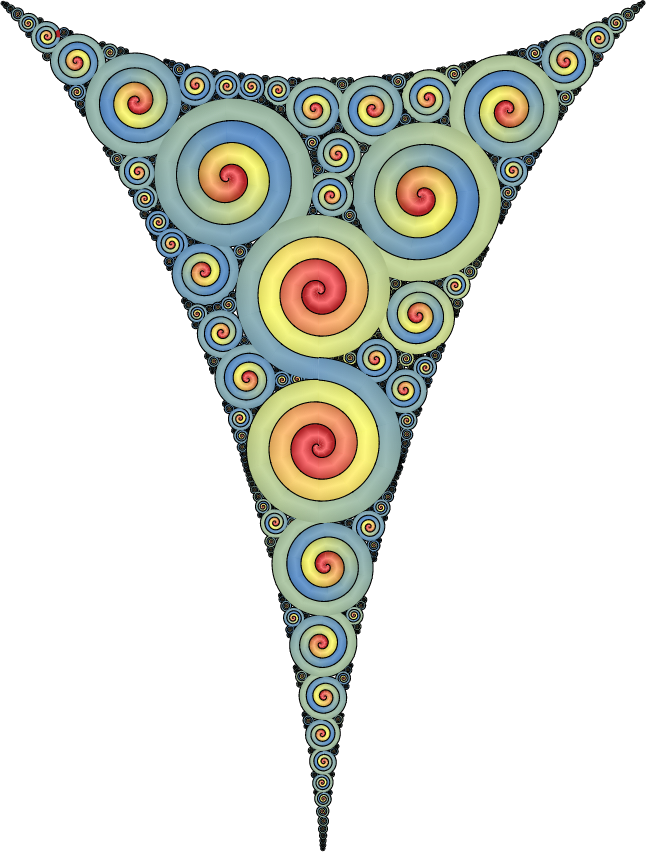
\includegraphics[width=0.75\linewidth]{pseudo-triangle}
\caption{Spiral packing inside of a pseudo-triangular boundary. A slight glass effect was added to give the colors depth. The image is vertically balanced, $B_{v} = -0.017$, with a high packing density, $porosity = 0.001$.}
\label{fig:pseudotri}
\end{figure}

When generating connected spiral sets, it was found that flipping orientation with each level of nesting gave best results, as the child spiral then generally followed its parent's direction of outward flow. In addition, boundary shapes with curves or tight pointed areas, such as the pseudo-triangle (Fig~\ref{fig:pseudotri}), found to give the best packing results.

The most attractive color schemes were found to be those that blended  around the spiral sweep such that there is some contrast between concentric layers. A constraint of coloring is that the children must exactly match their parent's color along the branch interval. If a child branches between two dominant parent colors, then its color scheme may benefit from some tweaking to avoid the diluting the color mix. Figure~\ref{fig:star} demonstrates this phenomenon; the seed spirals started out with a prominent red area where as children became progressively more green overall.

\begin{figure}[h]
\centering 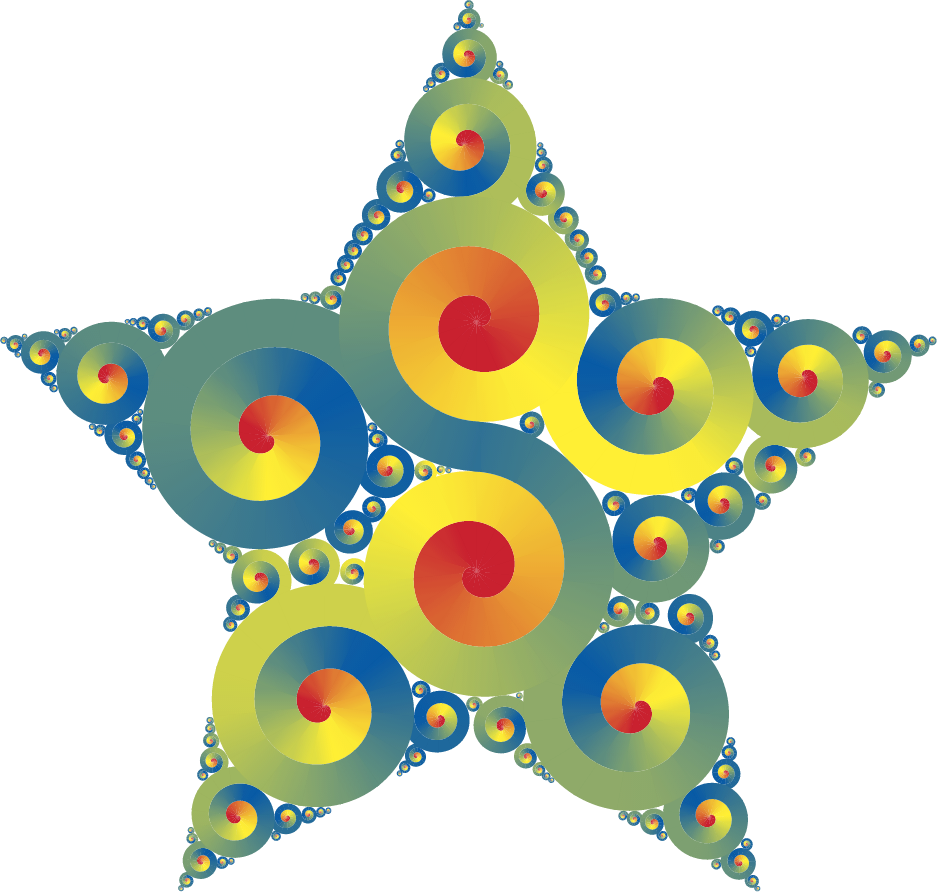
\includegraphics[width=0.75\linewidth]{star2}
\caption{Porous packing, $porosity = 0.013$, inside of a star boundary. No effect was added so the colors are flat. The image is slightly unbalanced to the right, $B_{v} = 0.109$ and fairly balanced over the horizontal, $B_{v} = 0.045$.}
\label{fig:star}
\end{figure}

\begin{figure}[h]
\centering 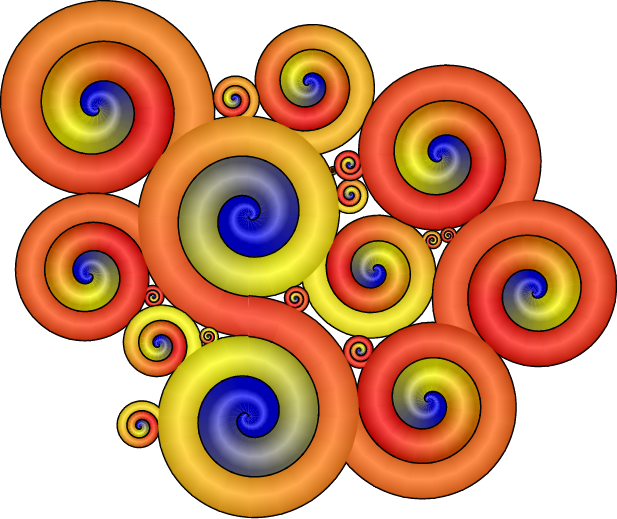
\includegraphics[width=0.75\linewidth]{noboundary}
\caption{An unbalanced connected set not packed within a boundary. Again, a slight glass effect was added to give the colors a bit of depth.}
\label{fig:nob}
\end{figure}

\label{results}

\section{Evaluation}
The algorithm aims to generate images that are both space-filling and visually pleasing, and so the output produced by the algorithm must be evaluated accordingly. The primary aspect evaluated was how space-filling the images were; the algorithm must produce an image with the packing density desired by the user. Secondly, the images must have a high aesthetic quality. Although this constraint is highly subjective, a number of programmatic techniques based on design principles were applied in an attempt to provide a good value of the aesthetic quality of the images produced.

\subsection{Packing Density}
The density of the packed images is measured by calculating the \textit{porosity}. This is the ratio of the vacant space to the filled space in the image. Therefore a lower porosity value indicates a tighter, more dense, packing, with zero being a completely filled area. In the case of spiral packing, the porosity is calculated as: 
\begin{equation} 
porosity = \frac{A_{bounding}}{\sum_{s \in spirals}A_{s}} - 1
\end{equation}
where $A_{bounding}$ is the area of the boundary shape and $A_{s}$ is the area of a placed spiral. An image with a lower calculated porosity is considered to be better packed. 

The implemented program calculates and displays the porosity as the user places spirals as an indication of the packing density.

\subsection{Design}
The design of the generated images is important when discussing the overall aesthetics of the images and how visually pleasing they are considered to be. As an attempt to programmatically quantify the visual quality of the images, two aspects of the design are considered: the balance and the color harmony. These two design aspects were chosen because they are particularly relevant to the images produced. Other design aspects, such as unity, texture and shape, are less relevant because the images do not use textures and are composed entirely of spiral shapes.

Balance, in general, is the distribution of the visual weight of objects, colors, texture, and space. In a well-balanced design, these elements are used in ways that make the design feel stable. Therefore, if an image exhibits good balance then it is generally considered more visually pleasing than an image exhibiting poor balance. For the purposes of evaluating the balance of the generated images, only the space that the spirals occupy (the area) is taken into consideration.

The balance about an axis of a generated image can be calculated as the difference in total spiral area on either side of a reference axis. For example, if we consider the center of the packing as $(\sum\frac{x_{s}}{n}, \sum\frac{y_{s}}{n})$, where $(x_{s}, y_{s})$ is the center of a spiral and $n$ is the total number of spirals that have been placed, then the vertical balance of an image would be the total spiral area to the left of the vertical axis through the center of the packing subtracted from the total area to the right. Dividing this value by the total area of all spirals would give a value in the range of $[-1, 1]$, where a negative value suggests a left-heavy image, a positive value suggests a right-heavy image, and a value of zero suggests a balanced image. Similarly, the horizontal balance would be the balance calculated with respect to the horizontal axis through the center of the packing, where the bottom area is subtracted from the top. A negative value would then suggest a bottom-heavy image, a positive value suggests a top-heavy image, and a value of zero suggests a balanced image.

Color harmony is another important aspect of visual design. It is defined as the pleasing arrangement of color within an image that engages the viewer and it creates a sense of order and balance in the visual experience. When an image is not harmonious, it is either boring or chaotic. Wei et al. show that the color schemes of packaging designs for fruit juice cartons impacted the consumers perception of the quality and freshness of the product. Carton designs that had harmony in color were perceived to be associated with a higher quality product.\cite{wei2014} There are many schools of thought when it comes to exactly what color arrangements and what aspects of color provide the best harmony. However it is generally considered true that images exhibiting color harmony of some sort are more pleasing than those without harmony of color. \cite{westland2007}

Therefore, the colors used in the generated images must harmonize in order for the image to be considered visually pleasing. The evaluation of color assumes that color schemes perceptively close to the harmonious color schemes described in Section~\ref{implementation} are also harmonious. Therefore the color harmony of the resulting image is calculated as the minimum perceptible difference between the colors chosen by the user and each of the harmonious schemes. The perceptible difference, $\Delta E_{ab}^{*}$, between two colors is determined using the CIE76 formula defined by the International Commission on Illumination (CIE), defined as: 
\begin{equation}
\Delta E_{ab}^{*} = \sqrt{(L_{2}^{*}-L_{1}^{*})^2 + (a_{2}^{*}-a_{1}^{*})^2 + (b_{2}^{*}-b_{1}^{*})^2}
\end{equation}
where $(L_{1}^{*}, a_{1}^{*}, b_{1}^{*})$ and $(L_{2}^{*}, a_{2}^{*}, b_{2}^{*})$ are two colors defined in the $(L^{*}, a^{*}, b^{*})$ color space. Though the CIE76 difference formula was superseded by more advanced formulas to better account for saturated colors, the CIE76 proved good enough for our purposes while remaining computationally efficient.
 
The vertical and horizontal balance values as well as the color harmony value are displayed by the program to the user during the packing process to provide an indication of the image's overall aesthetic quality.

% Future work
\section{Future Work}
\label{future}
There are a number of ways for extending the spiral packing method presented. The most obvious next step would be to automate the packing process. This would require the program be able to detect the optimal location to place a child spiral. Browne and van Wamelen propose two potential ways to accomplish this\cite{Browne2006834}: 
\begin{enumerate}
	\item An \textit{image based} technique where the spiral footprint of each spiral placed is removed from the image and a distance map of the image is maintained to determine the optimal location, and 
	\item A technique based on \textit{polygonizing} the boundary area to determine its Constrained Delaunay Triangulation where each new spiral?s center is added as a vertex and the boundary retriangulated.
\end{enumerate}
In addition, automation would require expanding the programmatic evaluation of the visual design to include all of the commonly considered aspects, instead of just the two described above, in order to provide a more accurate representation of the aesthetic quality. 

Another candidate for future work would be to implement the exact geometric solution for the spiral fitting problem. Though this is much more complex, it would allow for accurate packings to an arbitrary density.

% Conclusion
\section{Conclusion}
\label{conclusion}
Cameron Browne and Paul van Wamelen present a simple iterative algorithm for creating artistic, space-filling designs based on spiral packings. By utilizing circles as an approximation to spirals, their algorithm provides a practical and much more simple solution to the spiral packing problem. In this paper we described this method for creating connected spiral sets in detail, used the implemented algorithm to generate images based on spiral packing, and provided a method of evaluating the space-filling and aesthetic properties of the resulting images. 


% References
\bibliographystyle{plain}
\bibliography{references}{}


\clearpage
\onecolumn

\section*{Appendix A: Algorithms} 
\label{app:A}

\begin{algorithm*}
\caption{General fitting algorithm for cases I, II, and III}
\label{alg:fitting}
\begin{algorithmic}
	\Require The child spiral $S_{0}$ centered at the preferred location with specified 
		      	number of turns $T$, width $w$, and orientation $\omega$.
	\Require The parent spiral $S_{1}$ to branch from.
	\Require The neighboring spirals $S_{2}$ and $S_{3}$ to fit to.
	\Ensure The fitted child spiral $S$
    	
	\Function{fit}{$S_{0}$, $S_{1}$, $S_{2}$, $S_{3}$}
		\State $S$ $\gets$ $S_{0}$
		\State $c_{0}$ $\gets$ circle centered at $S_{0}.center$ with
	         \State \hskip 10mm     radius equal to $w(T-1)$
	         \State $\Delta$ $\gets$ $+\infty$
	         \State
		         
	         \Repeat
		        	\State \textit{// Approximate the spirals as circles}
		        	\For{each spiral $S_{i = \{1,2,3\}}$ to be fitted to}
				\State $r_{i}$ $\gets$ radius of $S_{i}$ toward $S.center$
				\State $r_{si}$ $\gets$ radius of $S$ toward $S_{i}.center$
				\State $r_{so}$ $\gets$ $S.width * (S.sweep - 1)$
				\State $c_{i}$ $\gets$ circle centered at $S_{i}.center$ with radius $r_{i} - (r_{si} - r_{so})$
			\EndFor
			\State
				
			\State \textit{// Do the circle fitting}
			\If{no intersection} 
				\State Fit $c_{0}$ to $c_{1}$ 
			\EndIf
			\If{$S$ intersects only $S_{2}$} 
				\State Fit $c_{0}$ to $c_{1}$ and $c_{2}$ 
			\EndIf
			\If{$S$ intersects both $S_{2}$ and $S_{3}$} 
				\State Fit $c_{0}$ to $c_{1}$, $c_{2}$, and $c_{3}$ 
			\EndIf
				
			\State
			\State $\Delta$ $\gets$ difference in $c_{0}$'s new and previous centers
			\State $S.center$ $\gets$ $c_{0}.center$
			\State $S.width$ $\gets$ $c_{0}.radius/(T-1)$
		\Until{$\Delta$ $<$ threshold}
		\State \Return $S$
	\EndFunction
\end{algorithmic}
\end{algorithm*}
 % Fitting algorithm
\begin{algorithm*}
\caption{Spiral packing - Branching algorithm}
\label{alg:branch}
\scriptsize
\begin{algorithmic}[1]
	\Require $S_{P}$ - The parent spiral to branch off of.
	\Require $S_{C}$ - The preferred child spiral, including position, sweep, and orientation.
	\Ensure $S$ - A fitted spiral as close to the preferred child spiral as possible.
		
	\Function{branch}{$S_{P}$, $S_{C}$}
		\State $S$ $\gets$ $S_{C}$
		\State
			
		\If {$S.center$ inside $S_{P}$} 
			\State \Return error
		\EndIf
		\State
      
		\If {$S.width > S_{P}.width$}
			\State $S.width \gets S_{P}.width$
			\State $S.center$ $\gets$ new center in same direction as initially indicated by $S_{C}$
		\EndIf
		\State
			
		\If {$S$ does not intersect neighboring (non-parent) spirals}
			\State \Return $S$
		\EndIf
		\State
			
		\If{$S$ intersects 2 or more neighboring spirals}
			\ForAll{non-parent spiral}
				\State $D_{C}$ $\gets$ the current non-parent spiral approximated as a disk
				\State $D_{P}$ $\gets$ $S_{P}$ approximated as a disk
				\State $D$ $\gets$ the disk touching $D_{C}$ and $D_{P}$ with its center	on the
				\State \hskip 10mm  line connecting the centers of $S_{P}$ and $S$
				\State $r$ $\gets$ radius of $D$
				\State $S_{1}, S_{2}$ $\gets$ the two spirals with the smallest $r$ values
			\EndFor
			\State

			\State $S_{3}$ $\gets$ the spiral fitted to $S_{1}$ and $S_{2}$
			\While{$S_{3}$ intersects neighboring spirals}
				\State $S_{4}$ $\gets$ spiral with the largest intersection with $S_{3}$
				\State $S_{5}$ $\gets$ spiral fitted to $S_{1}$ and $S_{4}$
				\State $S_{6}$ $\gets$ spiral fitted to $S_{2}$ and $S_{4}$
				\State $S_{3}$ $\gets$ $S_{5}$ or $S_{6}$, whichever has the smallest width
				\State
					
				\If{the width of $S_{3}$ increased}
					\State \textbf{break}
				\Else \If{$S_{5}$ was selected}
					\State $S_{1}, S_{2} \gets S_{1}, S_{4}$
				\Else
					\State $S_{1}, S_{2} \gets S_{2}, S_{4}$
				\EndIf
				\State
						
				\State $S_{3} \gets \textit{spiral fitted to $S_{1}$ and $S_{2}$}$
				\EndIf
			\EndWhile
			\State
				
			\State $V_{S3}$ $\gets$ the vector from the center of $S_{P}$ to the center of $S_{3}$
			\State $V_{S}$ $\gets$ the vector from the center of $S_{P}$ to the center of $S$
			\State $\theta$ $\gets$ the angle between $V_{S3}$ and $V_{S}$
			\If{$\theta \leq 12.5\degree$}
				\State \Return $S_{3}$
			\EndIf
		\EndIf
		\State
		
		\If {$S$ intersects exactly 1 neighboring spiral}
			\State $S_{1} \gets$ the intersected neighbor spiral
		\Else
			\State $S_{1} \gets$ bounding spiral with the smallest bounding radius, as above
		\EndIf		
		\State
			
		\State $S_{2} \gets \textit{spiral with the same width as $S$ branching from $S_{P}$ and touching $S_{1}$}$
		\If{$S_{2}$ does not intersect neighboring spirals} 
			\State $V_{S2} \gets \textit{the vector from the center of $S_{P}$ to the center of $S_{2}$}$
			\State $V_{S} \gets \textit{the vector from the center of $S_{P}$ to the center of $S$}$
			\State $\theta \gets \textit{the angle between $V_{S2}$ and $V_{S}$}$
			\If{$\theta \leq 12.5\degree$}
				\State \Return $S_{2}$
			\EndIf
		\EndIf
		\State
			
		\State $S_{2} \gets S$
		\While{$S_{2}$ does not intersect neighboring spirals}
			\State $S_{1} \gets \textit{spiral with biggest intersection to $S_{2}$}$
			\State $S_{2} \gets \textit{spiral branching from $S_{P}$, touching $S_{1}$, with its center}$
			\State \textit{~~~~~~~ on the line connecting the centers of $S_{P}$ and $S$}
		\EndWhile
		\State \Return $S_{2}$
	\EndFunction
\end{algorithmic}
\end{algorithm*} % Branching algorithm

\clearpage
\section*{Appendix B: Generated Images} 
\label{app:B}

\begin{figure}[H]
\centering 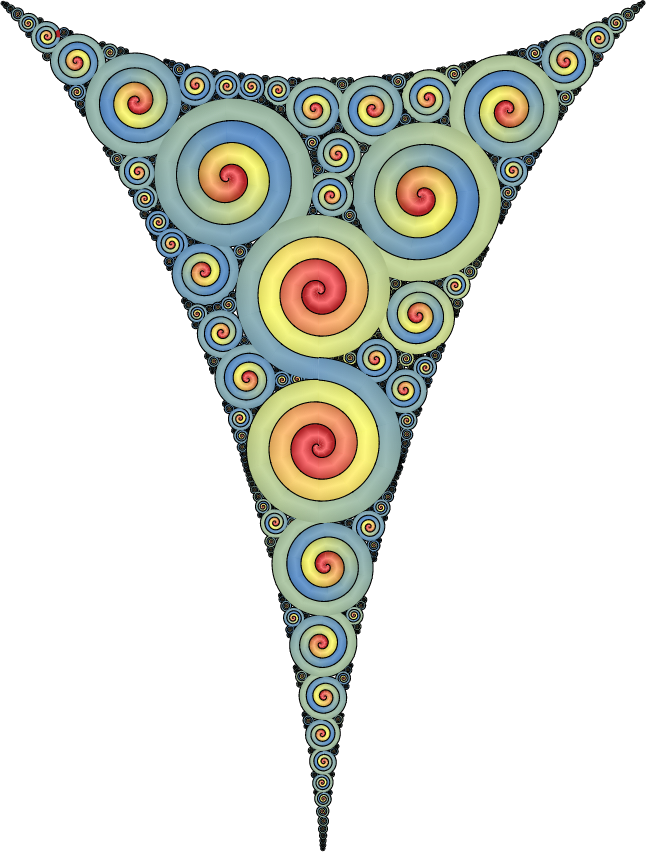
\includegraphics[width=0.8\textwidth]{pseudo-triangle}
\caption{Spiral packing inside of a pseudo-triangular boundary. A slight glass effect was added to give the colors depth. The image is vertically balanced, $B_{v} = -0.017$, with a high packing density, $porosity = 0.001$.}
\end{figure}

\begin{figure}[H]
\centering 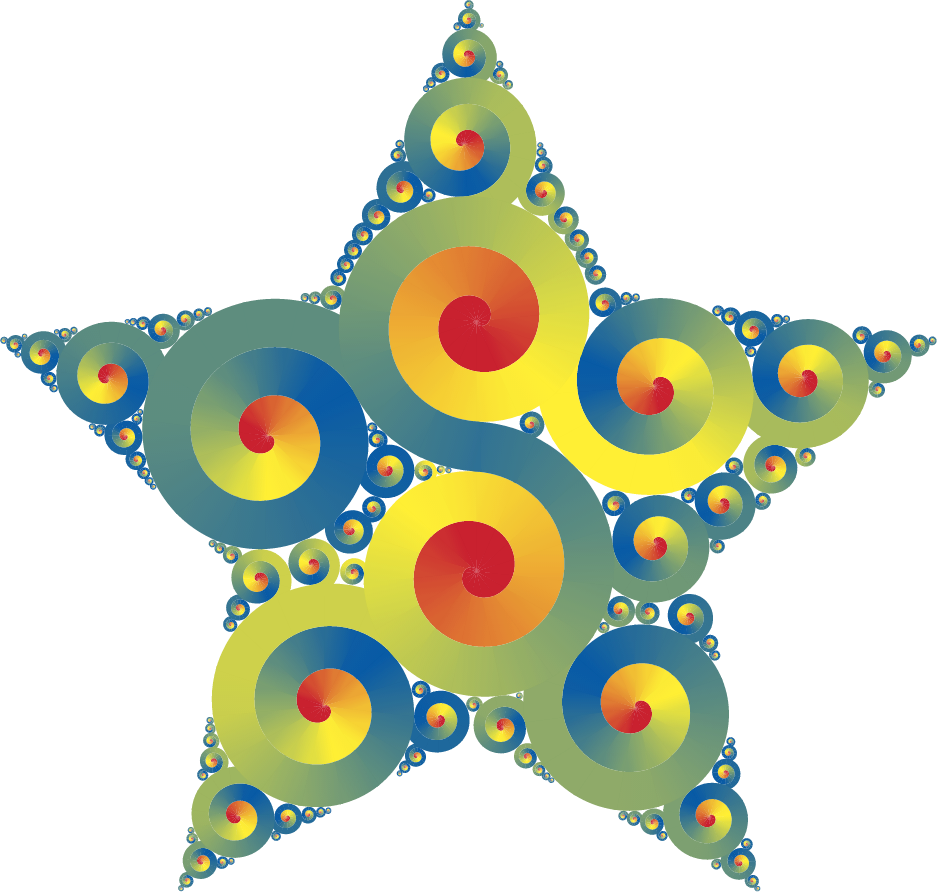
\includegraphics[width=0.8\textwidth]{star2}
\caption{Porous packing, $porosity = 0.013$, inside of a star boundary. No effect was added so the colors are flat. The image is slightly unbalanced to the right, $B_{v} = 0.109$ and fairly balanced over the horizontal, $B_{v} = 0.045$. Since the secondary colors are used, the color harmony is high, $H_{c} = 0.829$. }
\end{figure}

\begin{figure}[h]
\centering 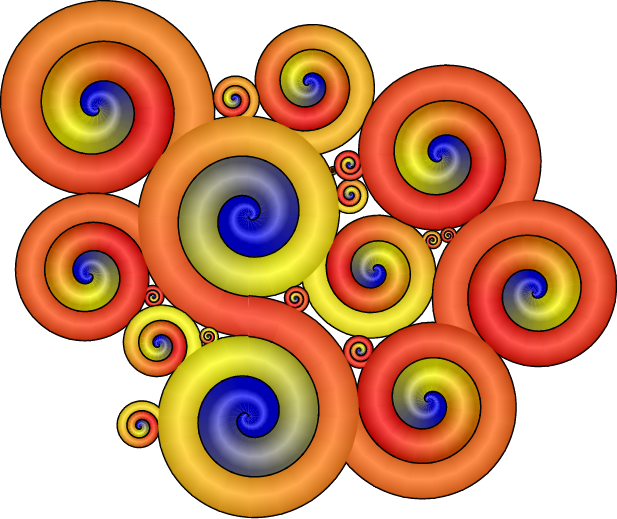
\includegraphics[width=0.8\textwidth]{noboundary}
\caption{An unbalanced connected set not packed within a boundary. Again, a slight glass effect was added to give the colors a bit of depth.}
\end{figure}

\end{document}



